% Template for IGARSS-2018 paper; to be used with:
%          spconf.sty  - LaTeX style file, and
%          IEEEbib.bst - IEEE bibliography style file.
% --------------------------------------------------------------------------
\documentclass{article}
\usepackage{spconf,amsmath,epsfig}
\usepackage{caption}
\usepackage{geometry}
\usepackage{setspace}

\special{papersize=8.5in,11in}
\captionsetup[boxed]{skip=6pt}
\setlength\parskip{0.1\baselineskip}
\oddsidemargin  -6.2truemm
\evensidemargin -6.2truemm

\topmargin 0truept
\headheight 0truept
\headsep 0truept
%\footheight 0truept
%\footskip 0truept
\textheight 229truemm
\textwidth 178truemm

\twocolumn
\columnsep 6truemm
\columnwidth 86truemm
% Example definitions.
% --------------------
\def\x{{\mathbf x}}
\def\L{{\cal L}}


% Title.
% ------
% Wind Directions Retrieval: A Method for Improving Accuracy of SAR Winds
\title{A Modified Circle Median Filter Method for Improving Accuracy of Wind Directions Retrieval from SAR Image}
%\title{Wind Directions Retrieval from SAR Image: A Method for Improving Accuracy of Winds}
%
% Single address.
% ---------------
\name{Yang Chao$^1$, Dongxiang Zhang$^1$, Kaijun Ren$^2$\sthanks{Corresponding author}, Jia Liu$^2$}
\address{$^1$National University of Defense Technology, College of Computer, Changsha 410073, China\\$^2$National University of Defense Technology, College of Meteorology and Oceanography,\\Changsha 410073, China}
%
% For example:
% ------------
%\address{School\\
%	Department\\
%	Address}
%
% Two addresses (uncomment and modify for two-address case).
% ----------------------------------------------------------
% \twoauthors
%   {Chao Yang, Dongxiang Zhang}
% 	{National University of Defense Technology\\
% 	College of Computer\\
% 	Changsha 410073, China}
%  {Kaijun Ren\sthanks{Corresponding author}, Jia Liu, Chaoxiong Ke}
% 	{National University of Defense Technology\\
% 	 College of Meteorology and Oceanology\\
% 	Changsha 410073, China}

\begin{document}
%\ninept
%
\maketitle
%
\begin{abstract}
Sea surface wind direction is extremely important for weather forecasts, oil spill monitoring, and so on. Up to now, wind direction retrieval from SAR images is stile difficult. There are two conventional methods of retrieving wind directions from SAR images, namely, two-dimensional fast Fourier transform (2D FFT) method and local gradients (LG) method. However, The spectral method works fine on open oceans, and large image areas, such as 20$\times$20km. In this paper, a new method which combines wind direction retireved from 2D FFT and LG with a modified cycle median filter(CMF) is proposed for improving accuracy of 2D FFT-retrieved wind directions filed. With Comparing different wind direction resolution, the high performance of the new method is validated. With the new method, the resolution of FFT-retrieved wind directions can be improved to 3km$\times$3km.
\end{abstract}
%Dual-polarized SAR images have been collected at low to moderate wind speeds with {\it in situ} buoy winds to construct a dataset containing 674 matchup data. Based on the matchup data, we analyzed the relations of the normalized radar cross section (NRCS) at cross-pol with the sea surface wind speed and incidence angle.
\begin{keywords}
synthetic aperture radar, wind direction, cycle median filter, wind streak, wind direction resolution
\end{keywords}
%
\section{Introduction}
\label{sec:intro}

With high spatial resolution, synthetic aperture radar (SAR) has been one of the most efficient instruments to obtain sea surface wind (SSW) information over large areas. In 1986, {\it Gerling et al.}\cite{Gerling:1986ee} found that the linear struction in the SAR image is related to the wind direction(WD) and extracted the WD from SAR spectra. Besides, marine atmosphere boundary layer (MABL) rolls were also observed in SAR images as linear streaks which is consistent with WD\cite{Alpers:1994hy}. From then on, the wind streak associated with WD become the main approach to retrieve WD. 

The main methods of WD retireval from SAR including fast Fourier transforms(FFT)\cite{Vachon:1996uj}, wavelet transform(WT)\cite{Du:2003ga}, local gradients(LG) and so on. In 1996, {\it Vachon et al.} extracted WD through spetral analysis by FFT. But FFT has a weakness for small image, e.g 10km$\times$10km\cite{Zhou:2017ec}.In 2003, LG which extracts WD by acquisition of the orthogonal of the most frequent gradient direction is propose by {\it Koch et al.}. LG overcomes the shortcoming of FFT and works better than FFT on spatial sampling of 10km$\times$ 10km, even 1km $\times$ 1km. The WD from a SAR by FFT or LG exsit 180$^\circ$ ambiguity, but it can be removed referencing to weather model output, Doppler shift or land shadows\cite{Horstmann:2003eg,Zhang:2014cr}.

When retrieving WDs from a SAR image, the SAR image is divided into a set of wind vector cells(WVCs). The direction at each WVC is extracted by FFT or LG. However, there are some isolated impolses in WDs because of noise. The essense different of FFT and LG is that they represent information from frequency domain and spatial domain respectively. In this way, considering conbining the two information is meaningful. The cycle median filter(CMF) technique is frequently used for ambiguity removal in wind vector retrieval from scattermetter\cite{Shaffer:1991ei,Stiles:2002cq}. CMF select a  wind vector that is the closest vector to the ture wind out of a set of ambiguous wind vectors at each wind vector cell(WVC)\cite{Shaffer:1991ei}. In this way, CMF can be used to improve accuracy of FFT-retrieved WDs by combining LG-retrieved WDs from a SAR image. 

In this study, we use a modified CMF to improve FFT-retrieved WDs accuracy in a SAR image by combining LG-retrieved WDs that represent the direction from spatial domain. In addition, the method is tested in different WDs resolution with WD from National Data Buoy Center(NDBC).

The remaining sections are organized as follows. In section \ref{sec:data}, the data used in this study are introduced. In section \ref{sec:method}, our method is described in detail.The perfomance of the method is tested in different WDs resolutionn in section \ref{sec:result}. Conclusions are given in section \ref{sec:conclusion}
\section{Data}
\label{sec:data}
\begin{table*}[htpb]
 \setlength{\belowcaptionskip}{0.1cm}
% \setlength{\abovecaptionskip}{0.2cm}
\centering
% \footnotesize
\caption{Informations of SAR IW mode Images.}
  \begin{tabular}{ccccccc}
    \hline
    &Start Time&End Time&Center Lat&Center Lon&Ascending or Descending?\\
    \hline
    %S1A_IW_GRDH_1SDV_20170518T141604_20170518T141629_016637_01B9B7_C40C
    1&2017-05-18T14:16:04Z&2017-05-18T14:16:29Z&36.7694&-123.3518&Descending\\
    \hline
    %S1A_IW_GRDH_1SDV_20170518T233538_20170518T233603_016643_01B9E6_D58F 
    2&2017-05-18T23:35:38Z&2017-05-18T23:36:03Z&24.5454&-82.5721&Ascending\\
    \hline
    %S1A_IW_GRDH_1SDV_20170520T001818_20170520T001843_016658_01BA5D_566B 
   % 3&2017-05-20T00:18:18Z&2017-05-20T00:18:43Z&30.0685&-93.9963&Ascending\\
    %\hline
  \end{tabular}
  \label{tab:1}
\end{table*}

\begin{table*}[htpb]
 \setlength{\belowcaptionskip}{0.1cm}
% \setlength{\abovecaptionskip}{0.2cm}
\centering
% \footnotesize
\caption{Informations of {\it in suit} NDBC .}
  \begin{tabular}{ccccc}
    \hline
    Station&Latitude&Longitude&Wind Direction&Time\\
    \hline
    46012&37.363&-122.881&318&2017-05-18-14-20\\
    \hline
    plsf1&24.693&-82.773&97&2017-05-18-23-40\\
    \hline
  %  srst2&29.683&-94.033&129&2017-05-20-00-20\\
   % \hline
  \end{tabular}
  \label{tab:2}
\end{table*}
Sentinel-1 wide swath(IW) mode Ground Range Detected (GRD) Vertical-Vertical (VV) polarization SAR images can be downloaded from European Space Agency (ESA) Sentinels Scientific Data Hub with nominal resolution of 20m$\times$22m and pixel spacing of 10m in range and azimuth, respectively. In this study, we concentrate on WDs retrieval from VV-polarized SAR image. Geometric calibrations are carried out by The Sentinel Application Platform 5.0 (SNAP 5.0)\cite{James:2017kn}.

Not all SAR images have wind streaks, so we select two Sentinel-1 IW mode SAR images in our study. Their informations are listed in Table \ref{tab:1}. Associated with SAR images, the {\it in situ} National Oceanic and Atmospheric Administration (NOAA) National Data Buoy Center (NDBC) buoys are collected, which are listed in Table \ref{tab:2}, including WD at the time.

\section{METHOD}
\label{sec:method}
For wind vector retrieval from scattermeter, a modified median filter is used to select a unique wind vector out of a set of ambiguous wind vectors at each WVC. In this study, we regard WDs extrated by FFT and LG as ambiguous WDs.

For a set of data $A$ with length of $N$ and circular data $x_i\in A,1 \le i \le N$, the median $y$ can be expressed as :
\begin{equation}
y = \mathop{\arg\min}_{x \in A}\sum_{i=1}^N|x - x_i|
\label{equ:1}
\end{equation}
Based on \ref{equ:1}, a median filter is implemented by constructing a fixed-length data window which is passed over the data and a set of median data is acquired. For a set of data $A$ with length of $N$, window length is setted as $M$. At step $j$, the data in the window is $D_j=\{x_d|j-h\le d \le j+h, h=M/2\}$. As in the following, the expresion of \ref{equ:1} can be rewrited as:
\begin{equation}
y_i  = \mathop{\arg\min}_{x\in D_j}\sum_{m=i-h}^{i+h}|x-x_m|
\label{equ:2}
\end{equation}
In order to imply median filter into SAR imag, extending \ref{equ:2} for two-dimentional data is necessary:
\begin{equation}
y_{ij} = \mathop{\arg\min}_{x\in D_{ij}}\sum_{m=i-h}^{i=i+h}\sum_{n=j-h}^{j+h}|x-x_{mn}|
\label{equ:3}
\end{equation}
where $D_{ij} = \{x_{pq} | i-h\le p \le i+h, j-h\le q \le j+h , h = M/2\}$ is the data in $M \times M$ window.

To get more accuracy WD filed is to consider the two-dimentional WD filed $W_{ij}=\{x_{ij}^1, x_{ij}^2|x_{ij}\in D_{ij}\}$, where each grid point $(i, j)$ has two WD value, which are asscociated with WDs assignd by FFT and LG algorithm. Let $F_{ij},L_{ij}$ be the set of FFT-retrieved WD and LG-retrieved WD at grid point$(i, j)$. Thus, 
\begin{equation}
W_{ij} = F_{ij}\cup L_{ij}\quad \text{for all } i, j
\label{equ:4}
\end{equation}
 Let $F_{ij}$ be the initial WD filed at $(i, j)$ grid . In this way, expression \ref{equ:3} can be writed for the median filters as:
\begin{equation}
y_{ij} = \mathop{\arg\min}_{x\in F_{ij}}\sum_{m=i-h}^{i=i+h}\sum_{n=j-h}^{j+h}|x-x_{mn}|
\label{equ:5}
\end{equation}

In the center of the filter window, we can get a set of median $\{y_{ij}\}$ of each Window. The modified CMF can be write as :
\begin{equation}
z_{mn}= \mathop{\arg\min}_{k=\{1, 2\}}\sum_{m = i-h}^{i+h}\sum_{n=j-h}^{j+h}|y_{ij} - x_{mn}^k|
\end{equation}
where $x_{mn}^k \in W_{ij}$.

For each window, the purpose is to select the WD that is closest to the median of the window at each grid point in $W_{ij}$. The $z_{mn}$ is the value from $W_{ij}$, which is closest to $y_{ij}$. In this way, we get a new WD filed $Z_{ij}^{*}=\{z_{mn}\}$. The $Z_{ij}^{*}$ is used to replace $F_{i,j}$, and the filter selection process continues for each grid point $(i,j)$ to create new $Z_{ij}^{*}$. The whole process is repeated to select a new $Z_{ij}^{*}$ untile $Z_{ij}^{*}=F_{ij}$.In addition, the WDs from LG or FFT have 180$^\circ$ ambiguity, it's essential to remove 180$^\circ$ ambiguty with WD from NDBC for both FFT-retrieved and LG-retrieved direcition.

In the WDs filed retrieved by FFT, the isolated impolse often happen because of the noise. For the smoothness and continuity of wind filed, it's useful to replace isolated impolse with median value directly, but it's statistical-based method. Our method that uses WDs from LG to replace the error directions from FFT is more meaningful. Besides, it's effective to improve the resolution of FFT-retrieved WDs.

\section{Result}
\label{sec:result}
The wind streaks don't appear in all regions of the SAR image, so we find the wind streak patterns in a SAR image and apply FFT and LG to the sub-images at these locations. Besides, 180$^\circ$ ambiguty should be removed by buoy WD after applying FFT and LG. The default window size of our method is 5 and the step that the window passing the data is 2.

The first SAR image listed in Tabel\ref{tab:1} and acquired by Sentinel-1 IW mode in VV polarization with a resolution of 20m is shown in Figure\ref{fig:1}a. The SAR image is shown in gray and the land in the SAR image has been masked out. Besides, Associated with the first SAR image, a {\it in suit} buoy is marked in red diamond in Figure\ref{fig:1}a. On a 44km by 44km sub-image that is indicated by green box in Figure\ref{fig:1}a, Figure\ref{fig:1}b shows the WDs computed by FFT in white color and LG in red color. WDs are computed from 10m pixels on a 5km grid. The blue arrow (318$^\circ$) in left-button is the WD from {\it in suit} buoy '416012'. The time of WD acquired by buoy is almost consistent with the time of SAR image acquired by Sentinel-1 (error is less than 5 minutes).In addition,the WDs here are in the same coordinate, in which the direction of the northward and eastward wind vector is 0$^\circ$ (or 360$^\circ$) and 90$^\circ$ respectively.

As illustrated in Figure \ref{fig:1}b, the FFT-retrieved WDs is aligned with wind streaks closer than LG-retrieved WDs. That's the reason why we use LG-retrieved WDs to improving accuracy of FFT-retrieved WDs, rather than the other way around. However, there are some isolated impulses in FFT-retrieved WDs because of noise. Figure \ref{fig:1}c is same as \ref{fig:1}b except the green arrow that is the WDs from our method. It's obvious that our method revise FFT-retrieved WDs.

In general, FFT is effective on 20km$\times$20km  WVC and the difficulty of extracting WD by FFT is inversely related to the size of WVC\cite{Koch:2004fq}. When the wind resolution increase, FFT-retrieved WDs has more and more impulses. As show in Figure \ref{fig:1}, our method is effective on 5km$\times$5km. In Figure \ref{fig:2}a, the second SAR image listed in Table \ref{tab:1} and a {\it in suit} buoy marked in red diamond is shown. Figure \ref{fig:2}b is a 37km$\times$33km sub-image indicated by green box in Figure\ref{fig:2}a. And the FFT-retrieved WDs in white color and WDs from our method in green color that are acquired on a 4km grid are illustrated in Figure \ref{fig:2}b. In Figure\ref{fig:2}b, the WDs from our method is almost covered by FFT-retrieved and the steps described in Section \ref{sec:method} just run once. Figure \ref{fig:2}c is the same region as Figure \ref{fig:2}b, but FFT-retried WDs and WDs from our method are both computed on a 3km grid. Note that, there are much more impulses in the FFT-retrieved WDs and we repeat twich the steps. In both 4km-grid and 3km-grid, our method shows a great performance. 

\begin{figure}[tpb]
\setlength{\belowcaptionskip}{-0.6cm}
\centering
\begin{minipage}[b]{0.48\linewidth}
  \centering
  \centerline{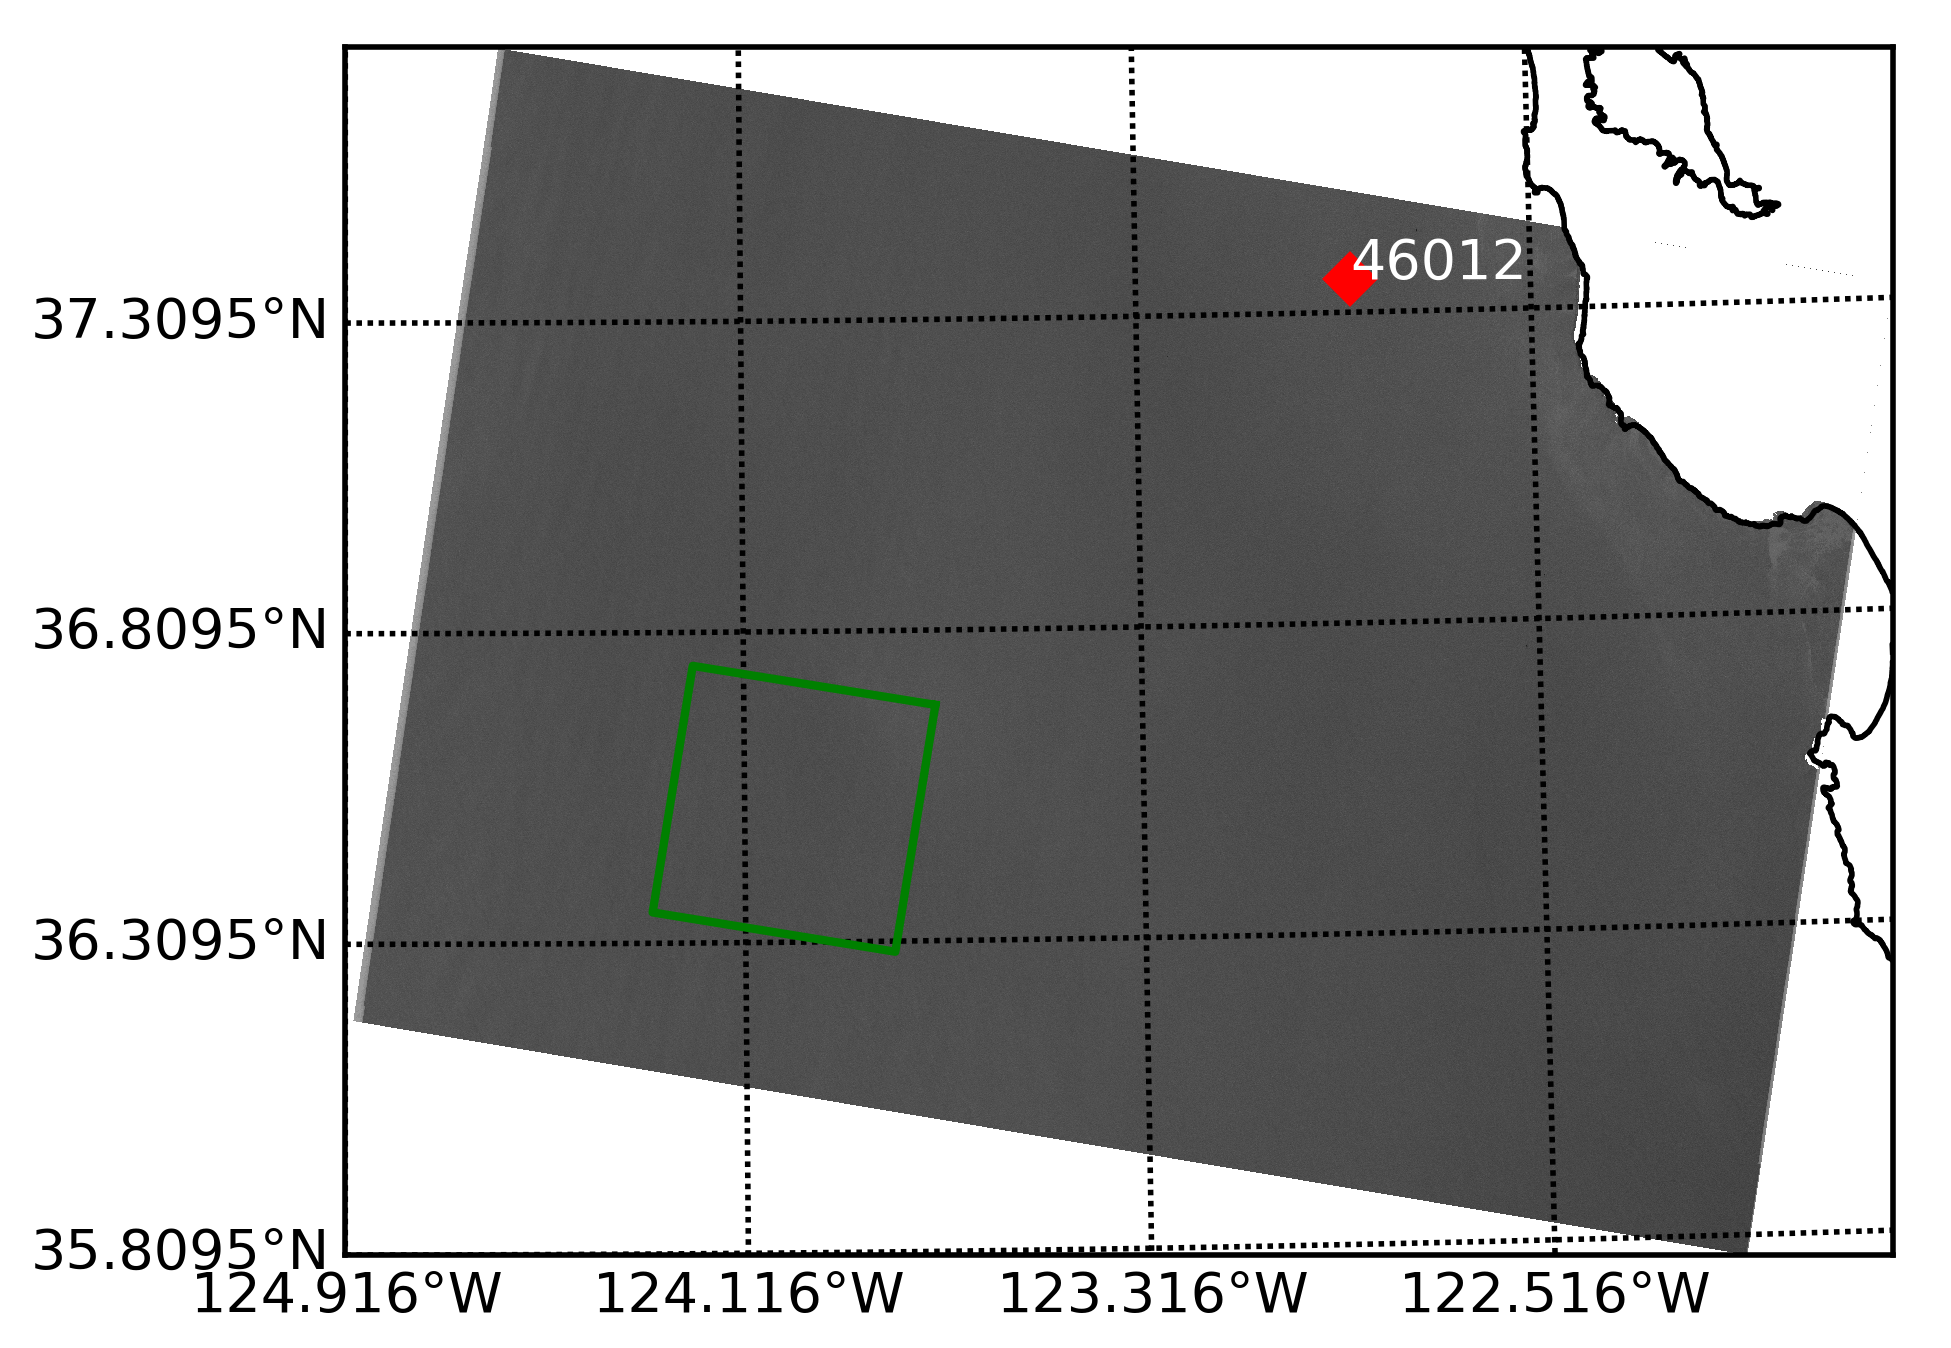
\includegraphics[width=8cm]{1.png}}
  \centerline{(a)}\medskip
\end{minipage}

\begin{spacing}{0.3}
\end{spacing}
%\vfill
% \begin{minipage}[b]{0.48\linewidth}
%   \centering
%   \centerline{\epsfig{figure=wspeedd1.eps,width=4.0cm}}
%   \centerline{(b)}\medskip
% \end{minipage}
\begin{minipage}[b]{0.48\linewidth}
  \centering
  \centerline{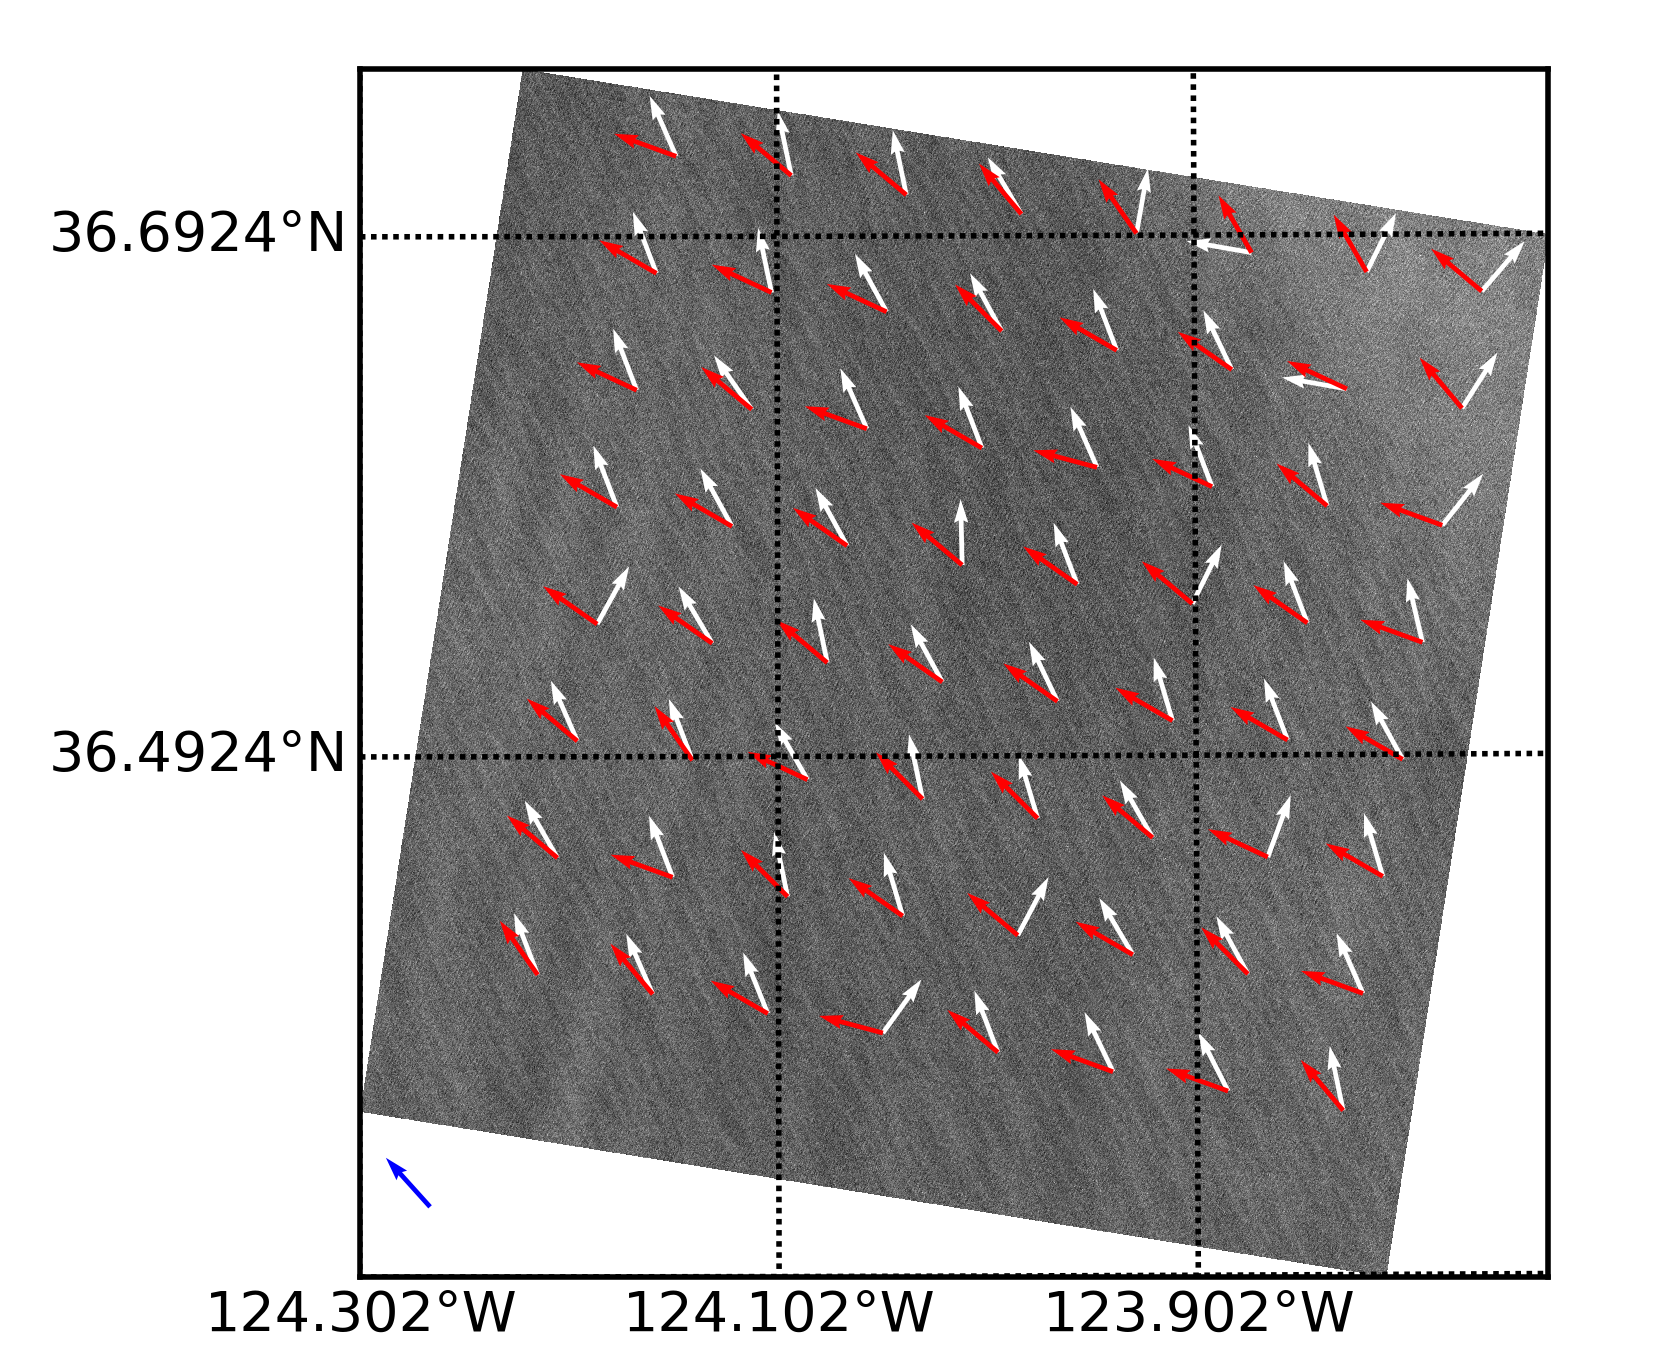
\includegraphics[width=8cm]{1_wind_5.png}}
  \centerline{(b)}\medskip
\end{minipage}
\begin{spacing}{0.3}
\end{spacing}
\begin{minipage}[b]{0.48\linewidth}
  \centering
  \centerline{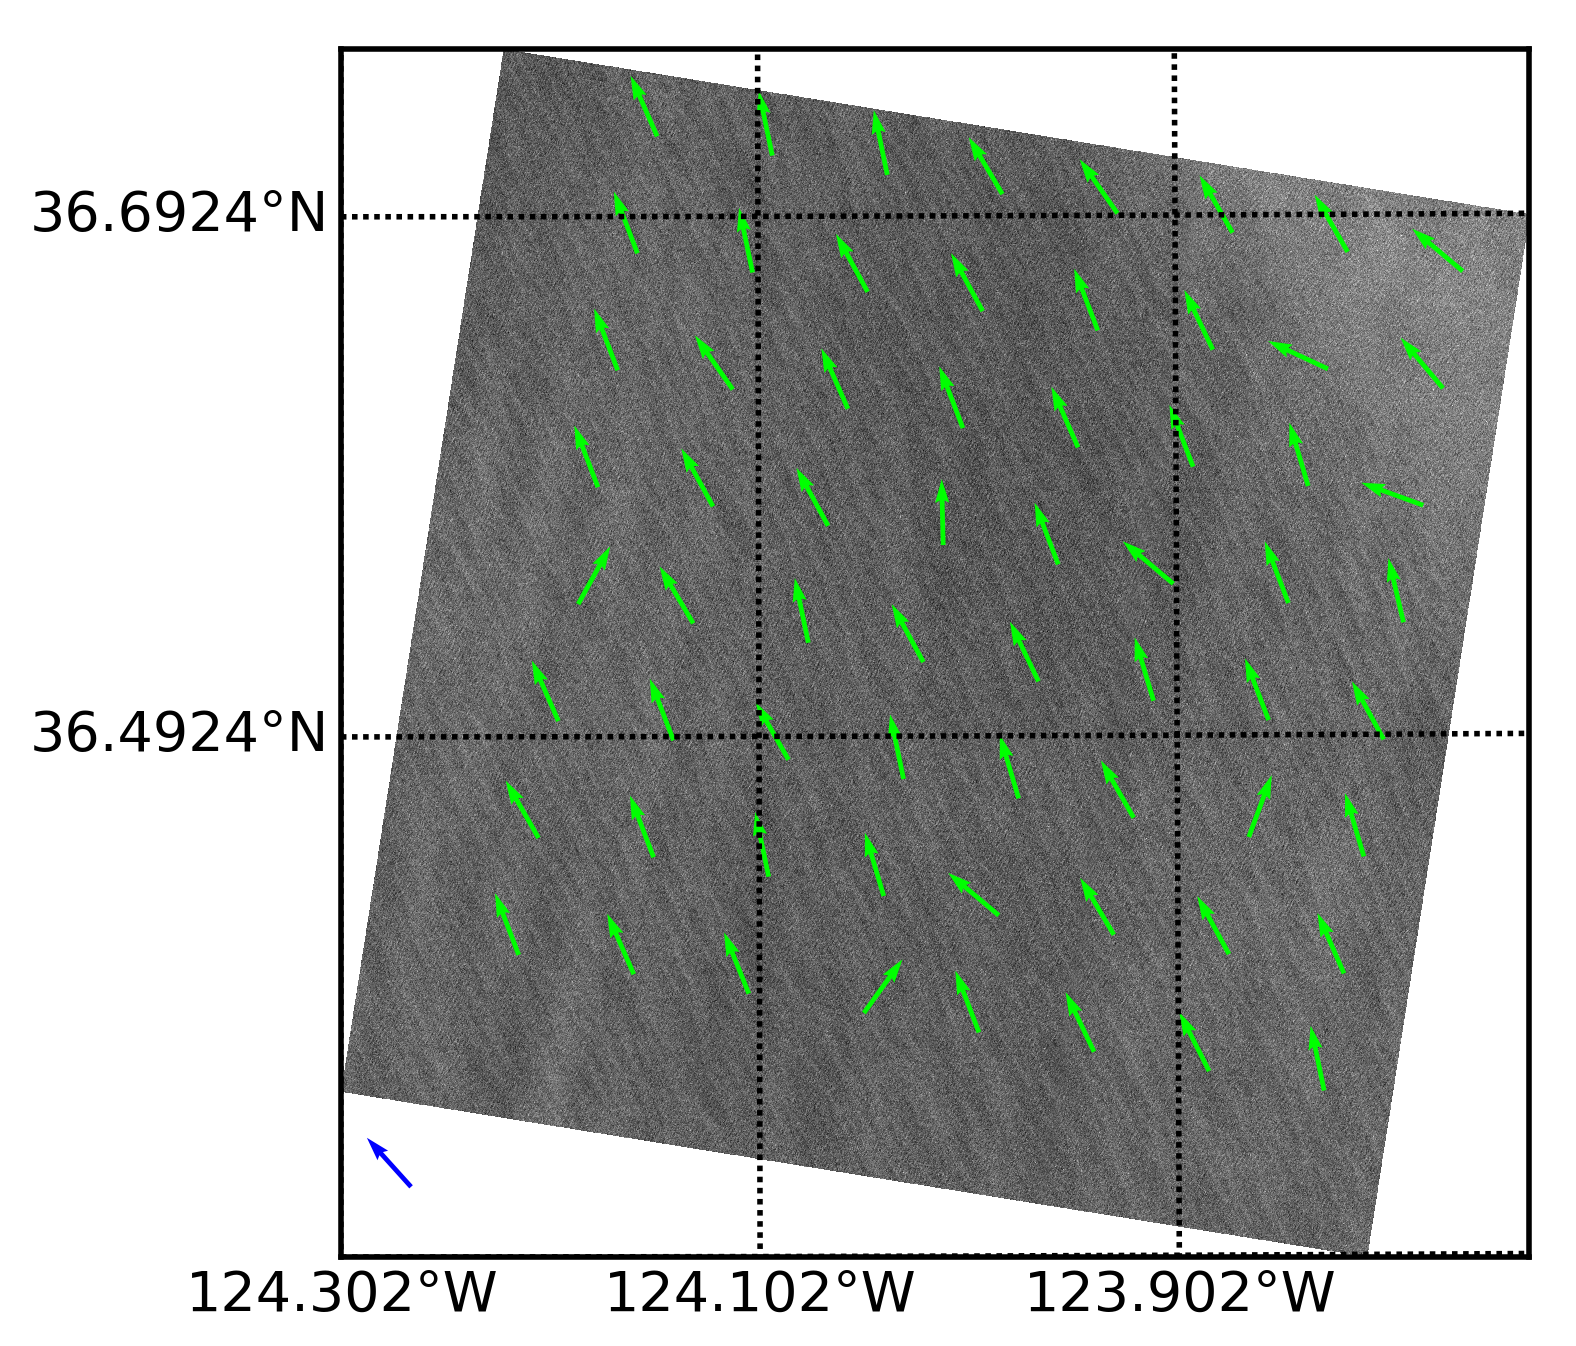
\includegraphics[width=8cm]{1_wind_m_5.png}}
  \centerline{(c)}\medskip
\end{minipage}
\setlength{\abovecaptionskip}{9pt}
\caption{(a) The first SAR image listed in Tabel\ref{tab:1} in VV polarization with a resolution of 20m. (b) The WDs computed from 10m pixels on a 5km grid by FFT in white color and LG in red color on a 44km by 44km sub-image that is indicated by green box in (a). (c)The WDs from our method on the same sub-image in (b).}
\label{fig:1}
\end{figure}

\begin{figure*}[tp]
\setlength{\belowcaptionskip}{-0.3cm}
\centering
\begin{minipage}[b]{0.32\linewidth}
  \centering
  \centerline{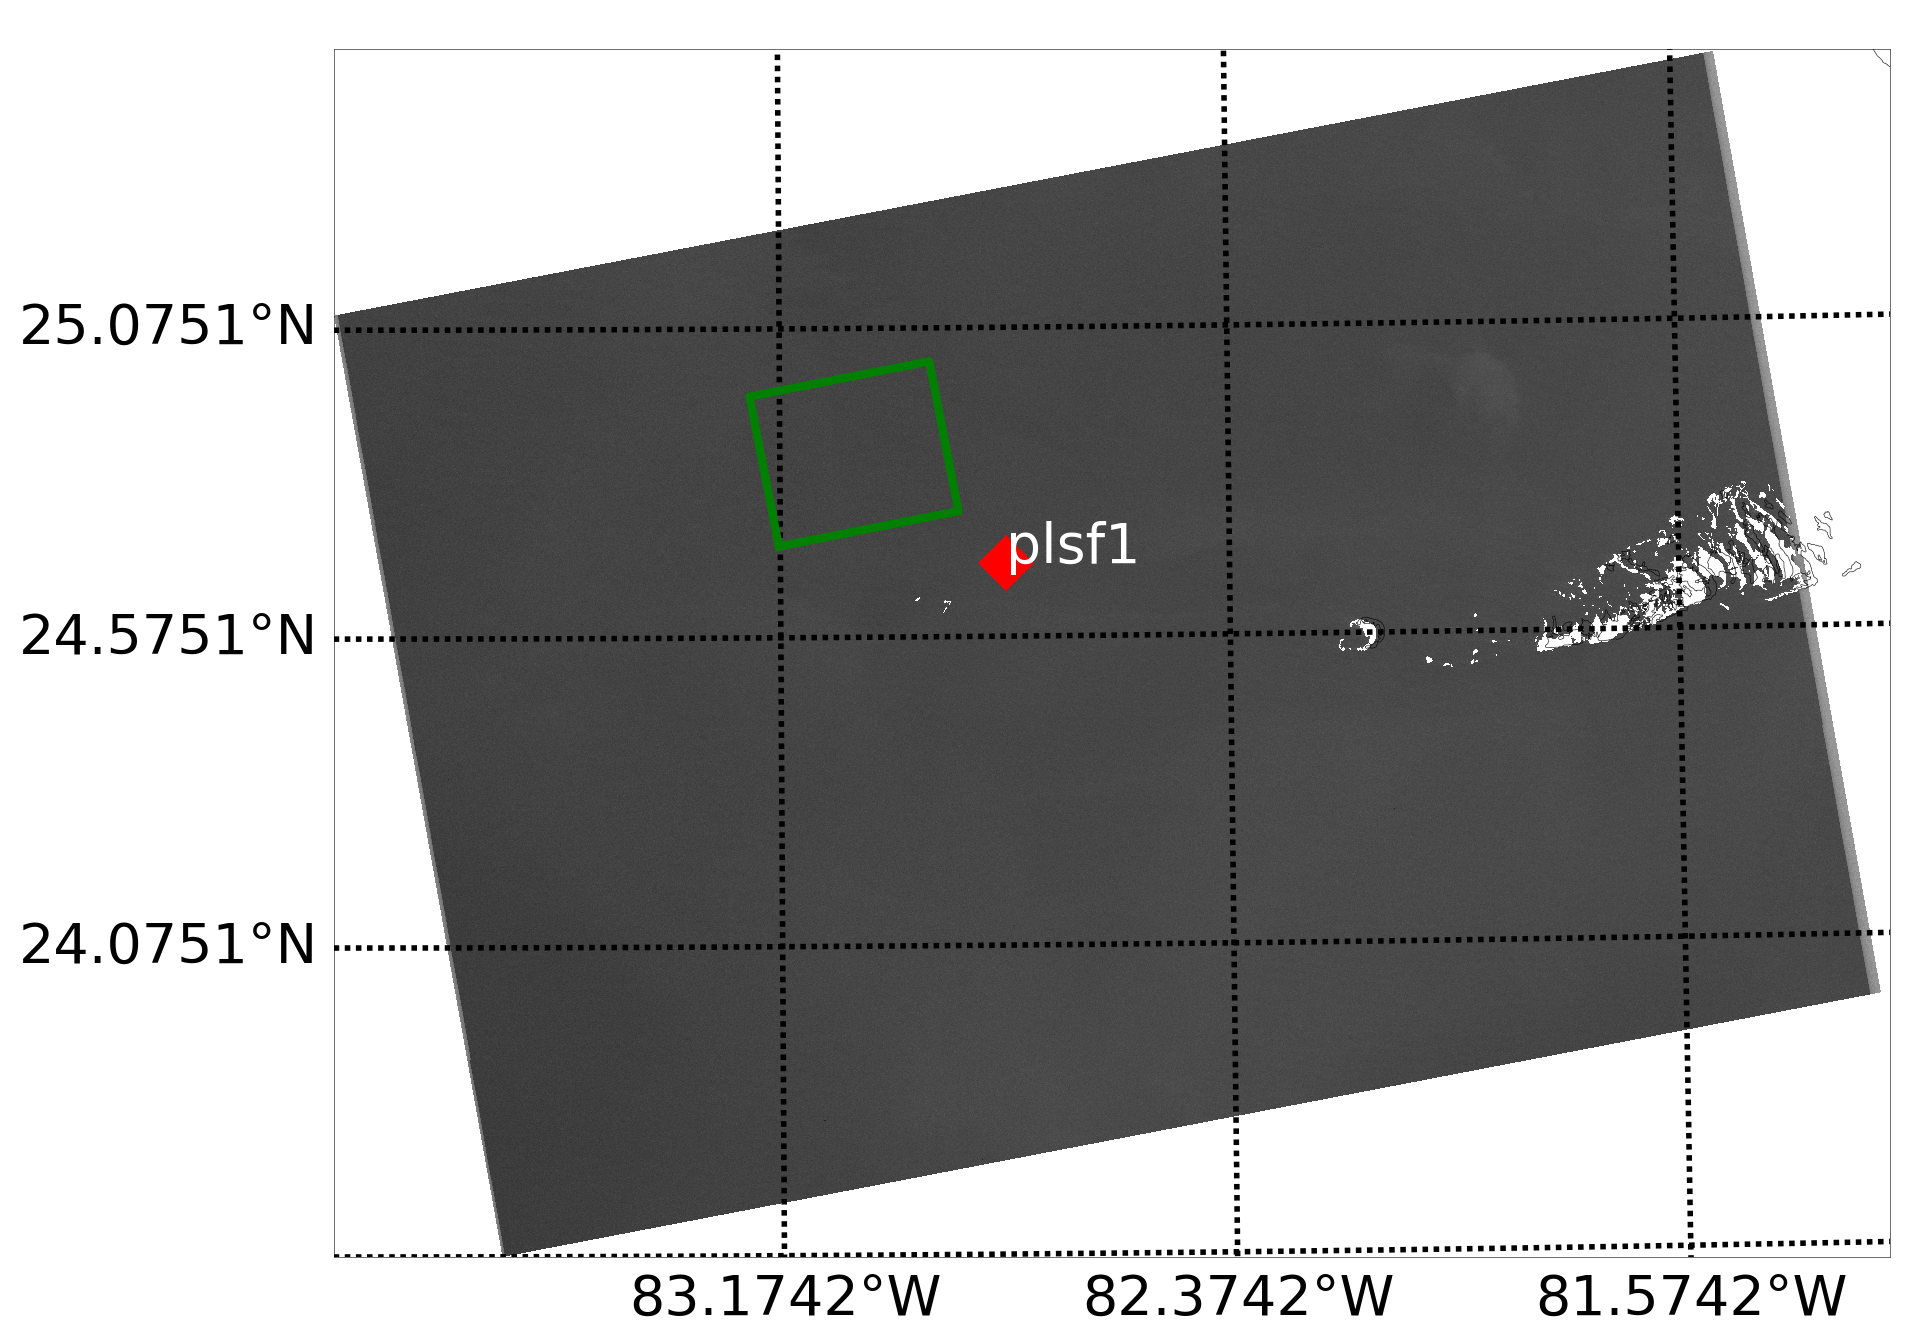
\includegraphics[width=6cm]{2.png}}
  \centerline{(a)}\medskip
\end{minipage}
% \vfill
\begin{minipage}[b]{0.32\linewidth}
  \centering
  \centerline{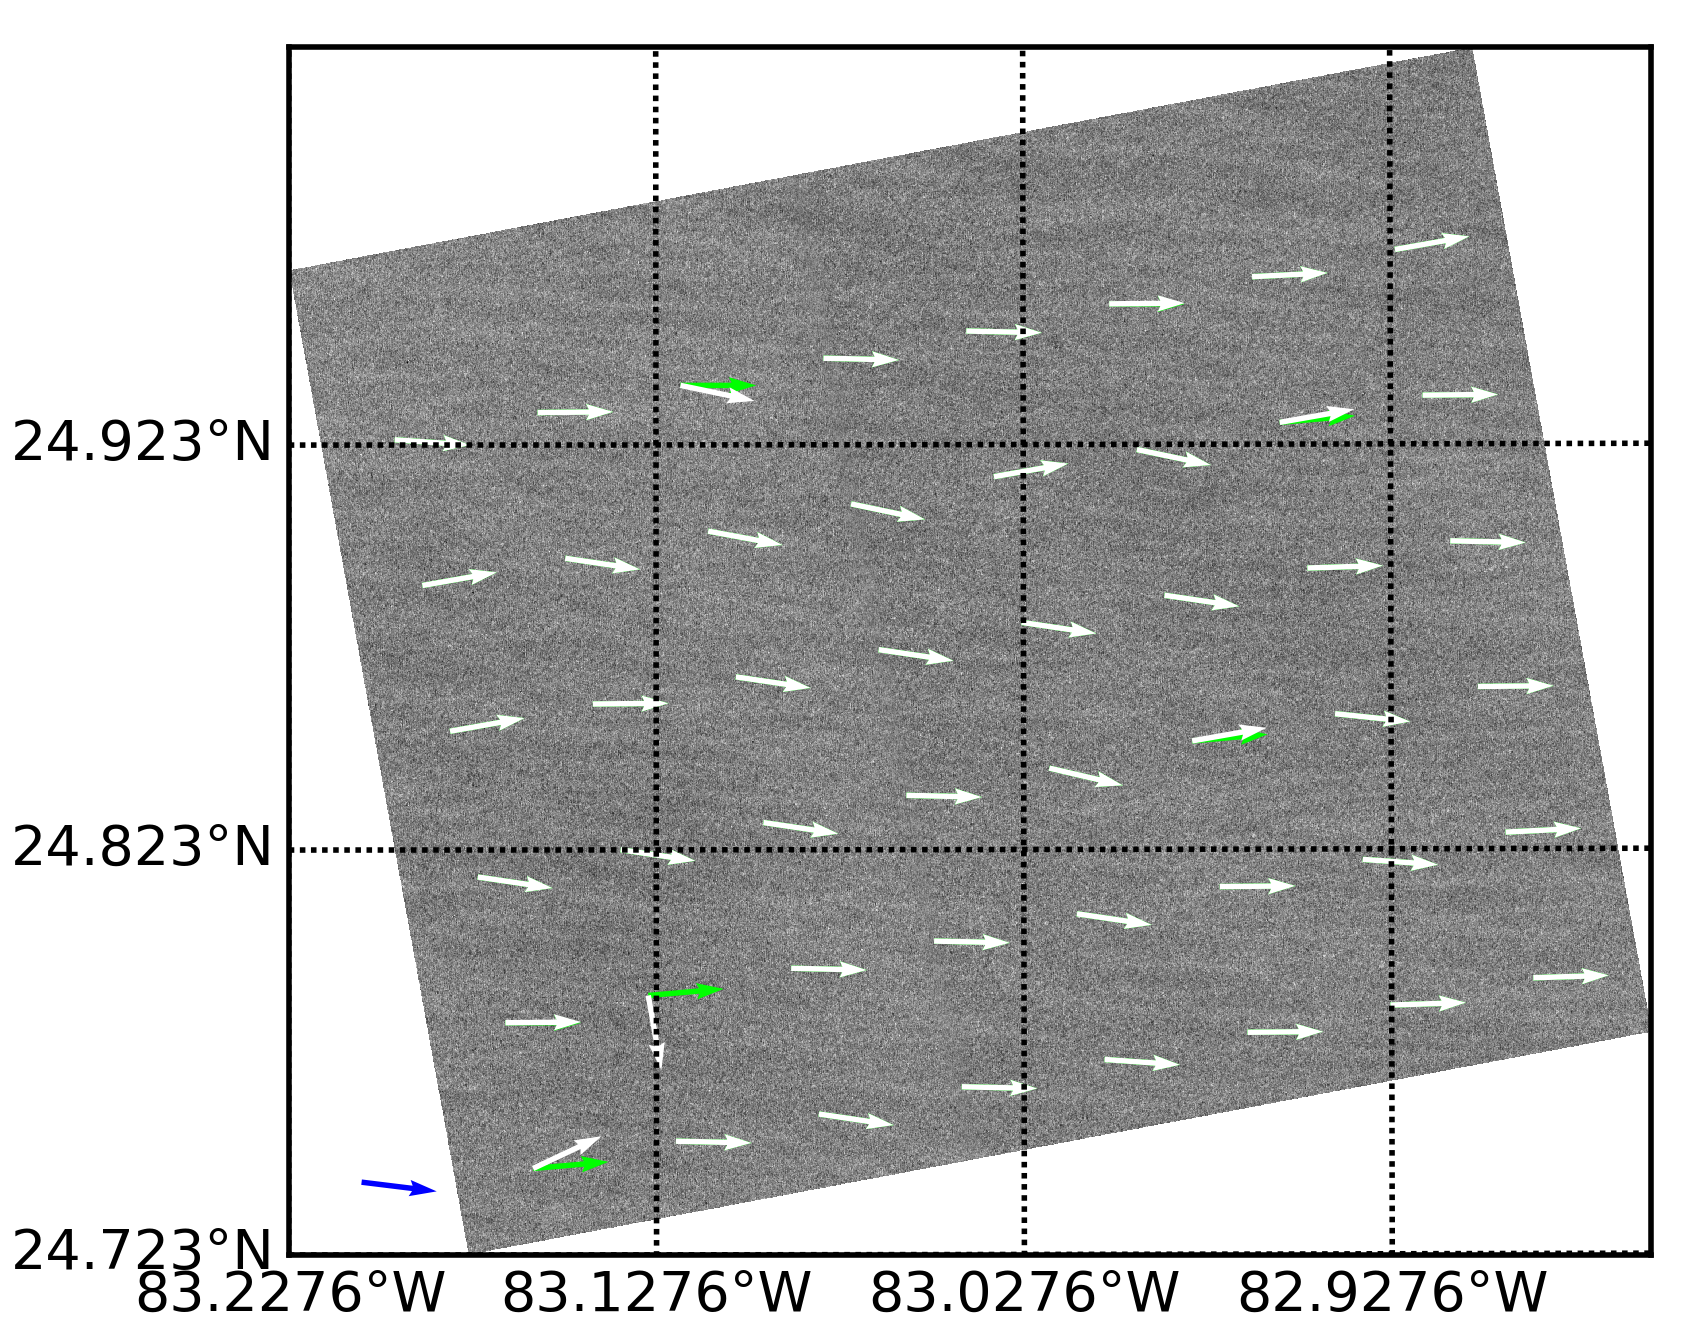
\includegraphics[width=5cm]{2_wind_a_4.png}}
  \centerline{(b)}\medskip
\end{minipage}
% \vfill
\begin{minipage}[b]{0.32\linewidth}
  \centering
  \centerline{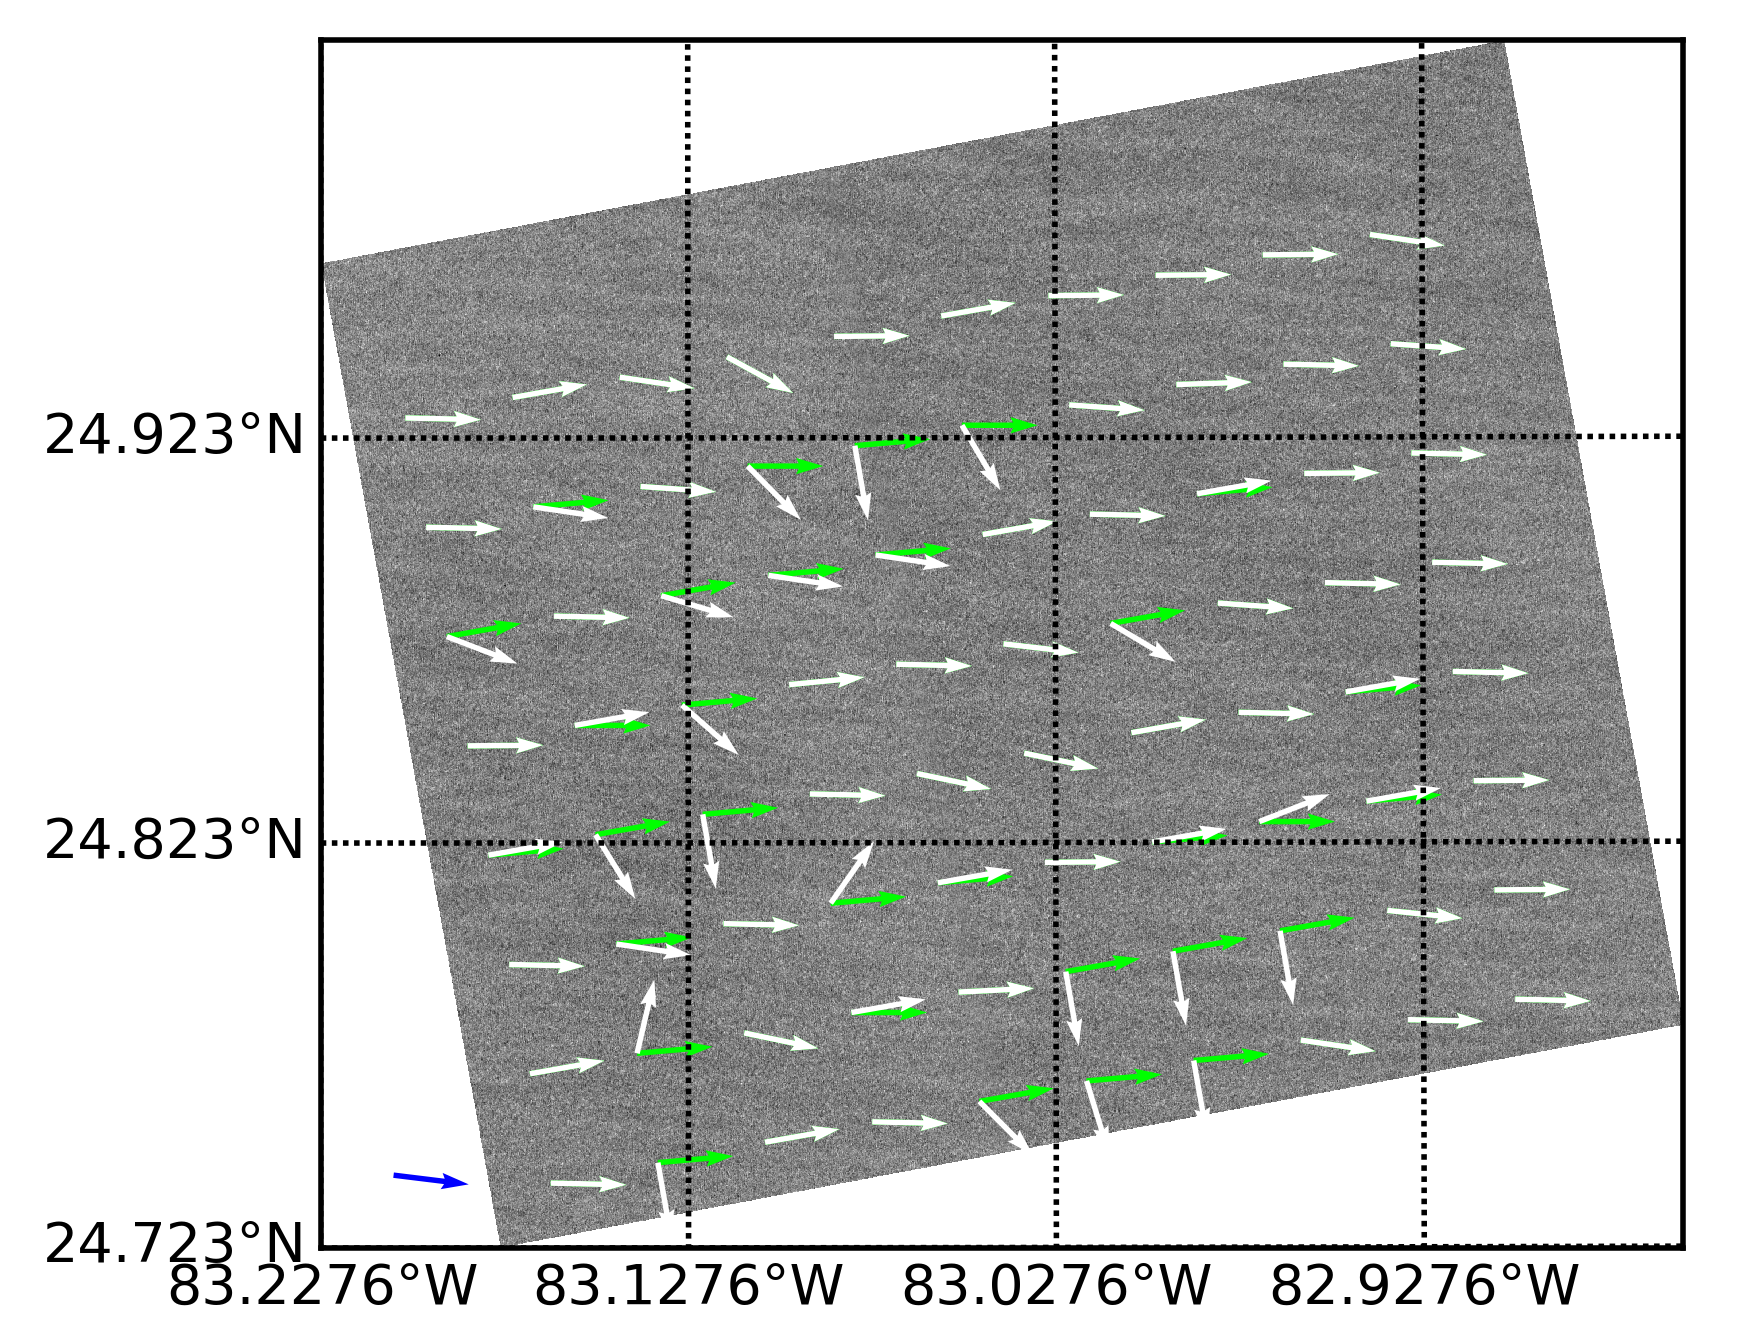
\includegraphics[width=5cm]{2_wind_a_3.png}}
  \centerline{(c)}\medskip
\end{minipage}
\setlength{\abovecaptionskip}{9pt}
\caption{(a) The second SAR image listed in Tabel\ref{tab:1} in VV polarization with a resolution of 20m. (b) The WDs computed from 10m pixels on a 4km grid by FFT in white color and our method in green color on a 37km by 33km sub-image that is indicated by green box in (a). (c)The WDs computed on a 3km grid by FFT in white color and our method in green color.}
\setlength{\belowcaptionskip}{9pt}
\label{fig:2}
\end{figure*}
CMF is always effective when over 50\% of the FFT-retrieved WDs are right. In fact, wavelengths of wind streaks is between 500m and 1500m\cite{Koch:2004fq}. When retrieve WDs from smaller region, The wind information can't be acquired from speckle domain of SAR image. Therefore, it's more difficult to retrieve WD when the grids become smaller. In Figure \ref{fig:3}, the FFT-retrieved WDs in white color are shown on a 1km grid and the results of our mehthod in green color has changed the mostly wrong directions. However, impulses are too many to revise. Therefore, the effective of our method is limited by the weakness of FFT.
\begin{figure}[htpb]
  \centering
  \centerline{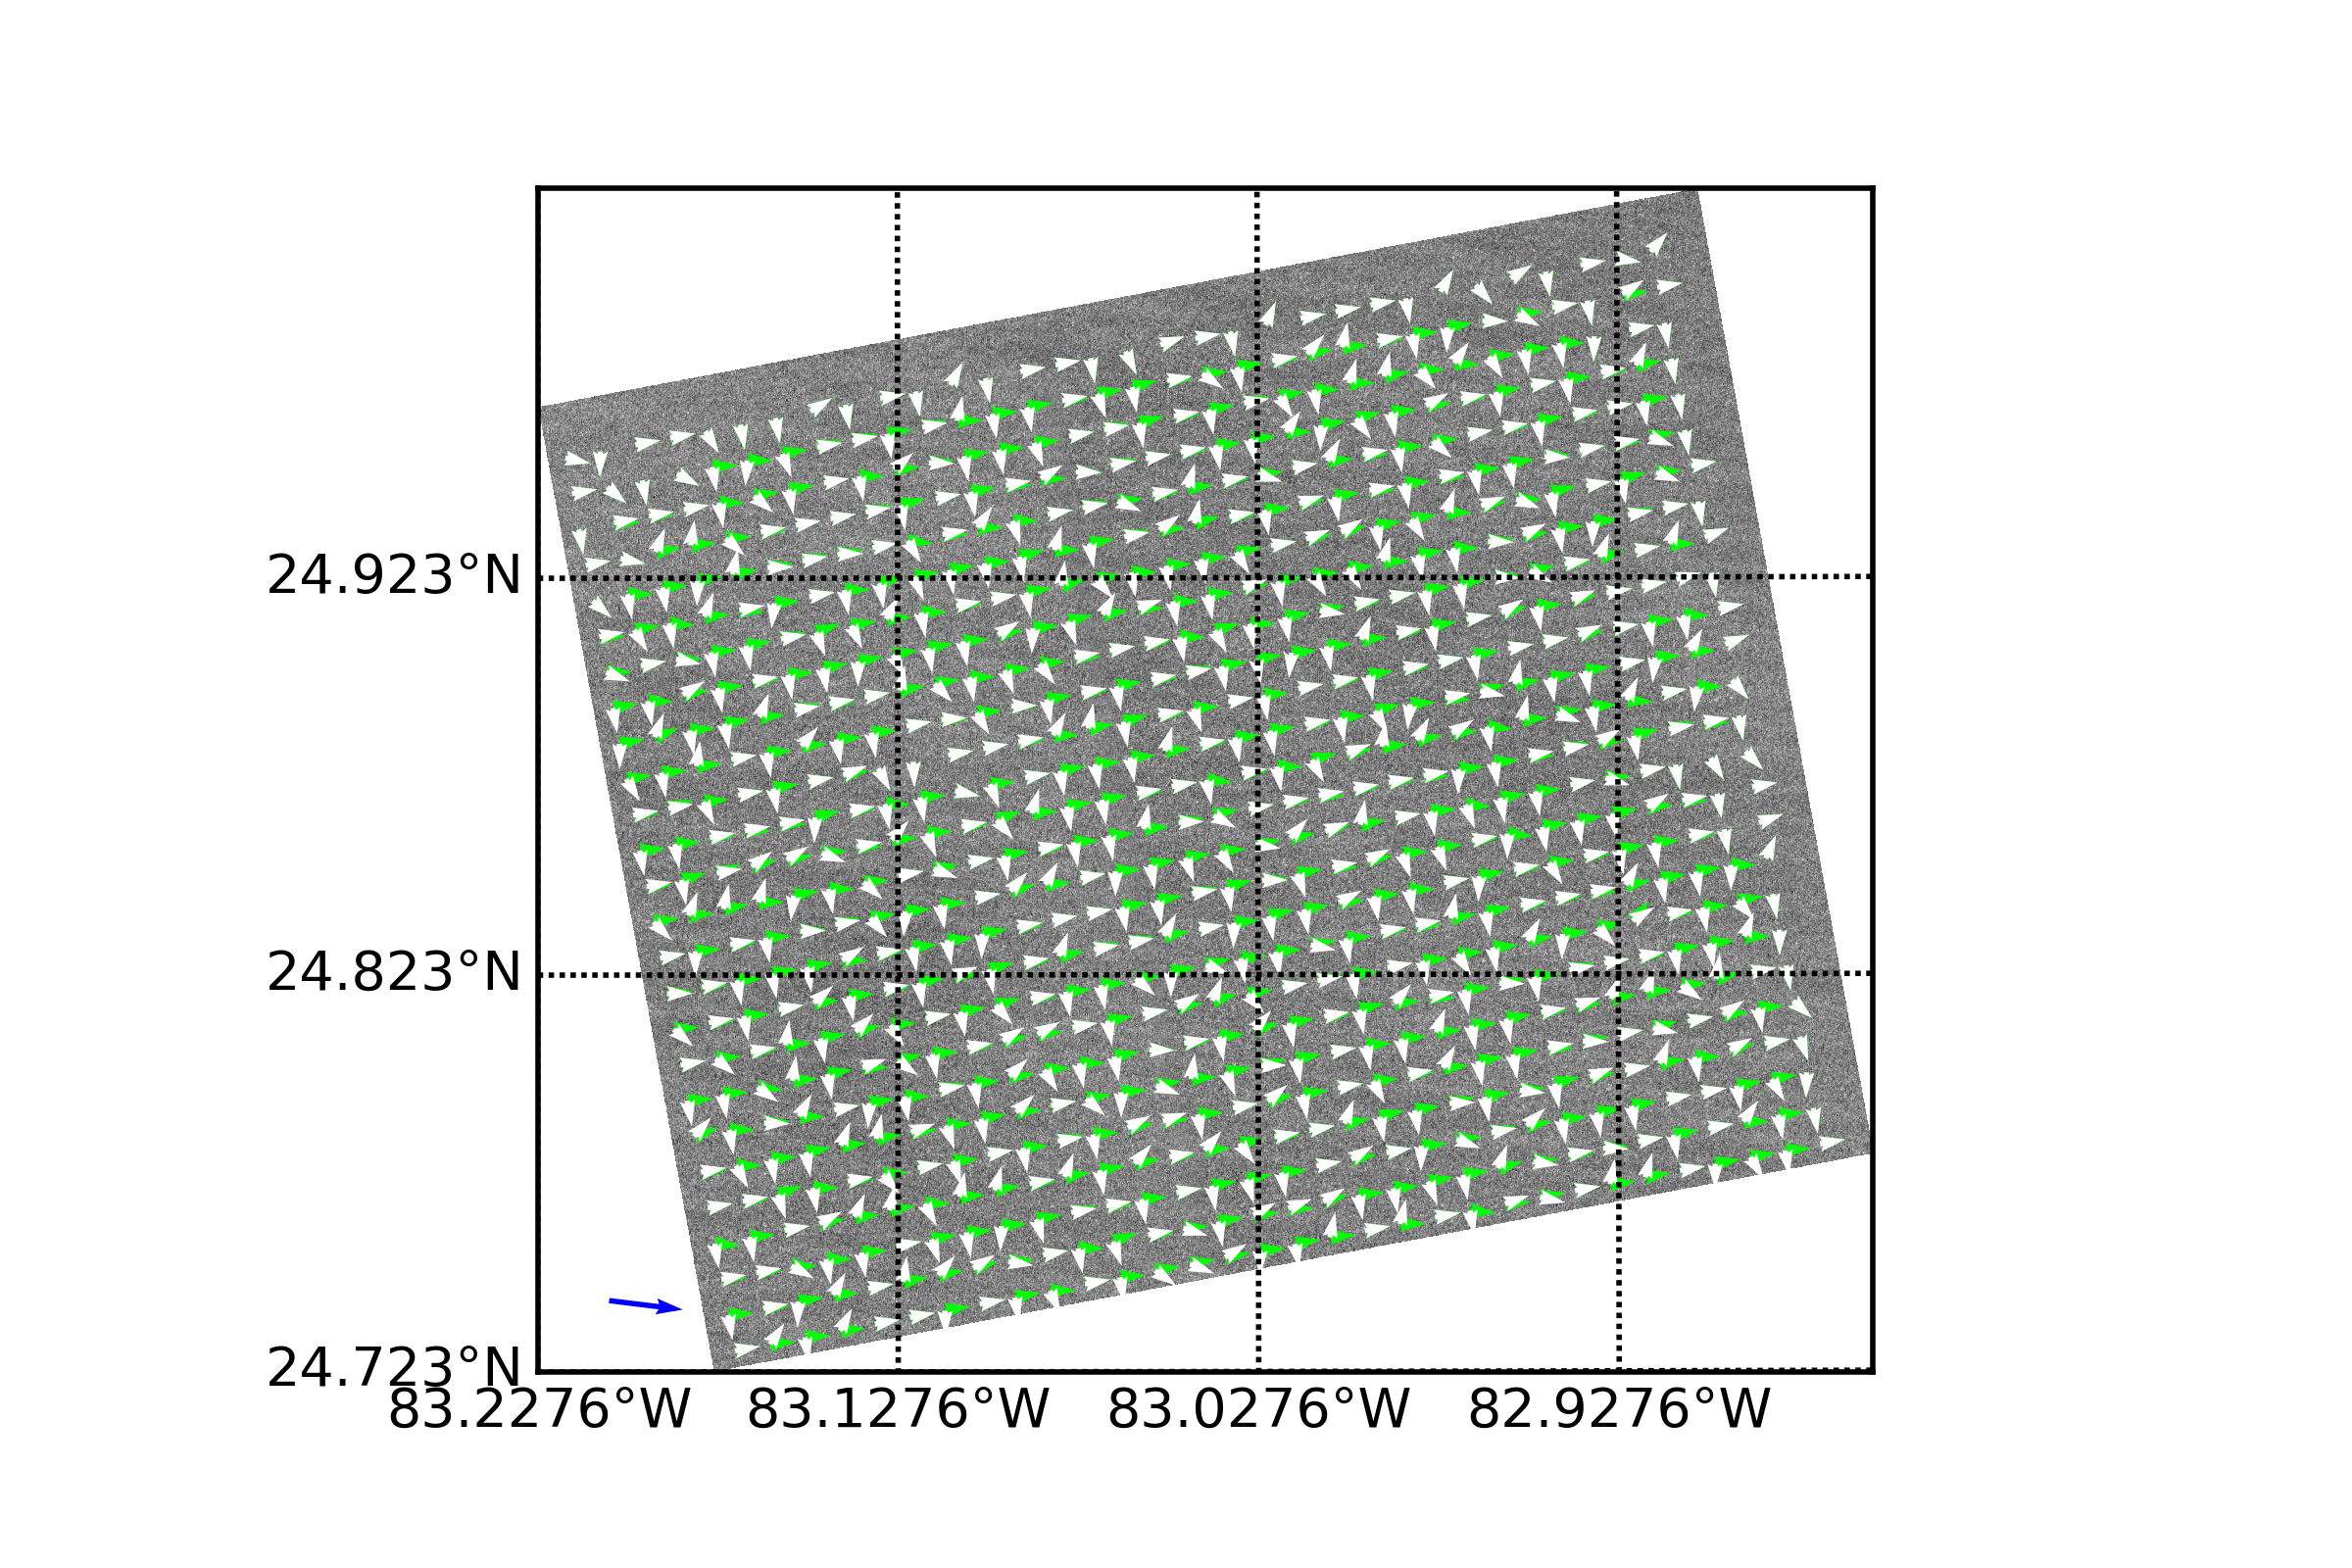
\includegraphics[width=0.48\textwidth]{2_wind_a_1_3.png}}
  \caption{The FFT-retrieved WDs in white color and WDs from our method in green color on a 1km grid on the sub-imge in Figure \ref{fig:2}b.}
  \setlength{\belowcaptionskip}{-0.3cm}
  \label{fig:3}
\end{figure}
\section{Conclusion}
\label{sec:conclusion}{}
In this paper, we concentrate on improving accuracy of FFT-retrieved WDs filed retrieved from SAR VV-polarized image by combining the FFT-retrieved directions and LG-retrieved directions. Considering the imformation of frequency domain and spatial domain, A modified CMF is proposed. 

In this work, we modified CMF to select the WDs that is closest to the ture WDs from FFT-retrieved WDs and LG-retrieved WDs. Two VV-polarized SAR image from Sentinel-1 IW mode are used to validate our method and the results show the effctive. Besides, we analyse the performance of our method in different WDs resolution. Since wavelength of wind streaks is between 500m and 1500m, the resolution of FFT-retrieved WDs is limited. With the WDs resolution increase, it's more and more difficult to retireve WDs filed using our method, which is caused by the weakness of FFT. However, our method can get higher WDs resolution than that from FFT. From our analysis, the new method have high performance in a 3km$\times$3km gird.

In addition, the filter size and step length of our modified CMF are not discussed in this work, and we use filter size of 5 and set lenght of 2 as default. One thing that has to point out is that many WD-retrieval methods can be used to replace LG in our method.In futuer works, we'll test them.

\section{ACKNOWLEDGEMENT} % (fold)
\label{sec:acknow}

This work was supported by the National Natural Science Foundation of China under Grant ****** . The Sentinel-1 SAR data and the SNAP 5.0 software are available through the European Space Agency Sentinels Scientific Data Hub and European Space Agency Step Scientific Toolbox Exploitation Platform.

% section section_name (end)
%61572510

% References should be produced using the bibtex program from suitable
% BiBTeX files (here: strings, refs, manuals). The IEEEbib.bst bibliography
% style file from IEEE produces unsorted bibliography list.
% -------------------------------------------------------------------------
\bibliographystyle{IEEEbib}
\bibliography{refs}

\end{document}
